\documentclass[conference]{IEEEtran}

\usepackage{amsmath}
\usepackage{graphicx}
\usepackage{booktabs}
\usepackage{array}
\usepackage{subcaption}
\usepackage{url}

% Upload the PNG files from Model Simulation/ to Overleaf alongside this .tex:
% aeris_dual_objective_snapshots.png
% aeris_dual_objective_metrics.png
% benchmark_dual_on_5seed.png
% benchmark_watch_off_5seed.png
% benchmark_watch_guarded_on_5seed.png

\title{AERIS Project Update: From Connectivity-Constrained ISR Simulation to Adaptive Multi-Axis Defense}

\author{
\IEEEauthorblockN{Jeewoo Choi}
\IEEEauthorblockA{
Stanford University\\
jchoi23@stanford.edu
}
}

\begin{document}
\maketitle

\begin{abstract}
The original AERIS proposal framed the project as a graph-based UAV autonomy
problem: dynamically assign UAVs to ISR, mobile relay, and static relay roles so
that useful ISR coverage is maximized while maintaining a communication path to
the operator. Since the proposal, the project has evolved from a primarily
visual proof-of-concept into a measurable simulation testbed. The current system
now includes connectivity-constrained ISR scoring, battery and recharge behavior,
enemy reactions, strike mechanics, dual undefended objectives, adaptive relay
branching, multi-seed benchmarking, and diagnostic plots. Recent experiments
show that branching improves the system's ability to address multi-axis threats,
but undefended north and south objectives still collapse under the current
policy. This update summarizes implemented progress, experimental findings, and
the next steps required to make the optimization behavior more decisive.
\end{abstract}

\section{Original Proposal Summary}
The proposal defined AERIS as an Autonomous Relay-Enabled ISR System for
resilient drone operations in contested environments. The key technical idea was
to model the UAV team as a dynamic graph where UAVs are nodes, communication
links are edges, and the base station is the root node. ISR data is counted as
valid only when the sensing UAV has a path back to the base.

The proposed role set was:
\begin{itemize}
    \item \textbf{ISR Mode}: collect surveillance data over the battlefield.
    \item \textbf{Mobile Relay Mode}: move while preserving communication links.
    \item \textbf{Static Relay Mode}: remain stationary as a stronger relay node.
\end{itemize}

The proposed optimization objective was:
\begin{equation}
\max \; w_1 C_{\text{ISR}}(t) + w_2 C_{\text{conn}}(t)
- w_3 E(t) - w_4 W_{\text{op}}(t) - w_5 N_{\text{switch}}(t),
\end{equation}
where ISR coverage is useful only when connected to the operator. The proposal
also introduced an FDIR-inspired autonomy loop: detect degraded conditions,
isolate their causes, and recover through role switching or repositioning.

\section{Implemented Since the Proposal}

\subsection{Discrete-Time Graph Simulation}
The current project implements the proposed discrete-time simulation loop. At
each step, UAVs move, batteries drain, enemies move, the communication graph is
rebuilt, connected UAVs are identified, valid ISR coverage is computed, and the
optimizer updates UAV roles and movement targets.

\subsection{UAV Role Switching and FDIR Behavior}
The simulator now supports ISR, mobile relay, static relay, return-to-base, and
recharge behavior. UAVs can be promoted from ISR to relay roles when the network
needs additional communication support. Mobile relays become static once they
reach assigned waypoints and satisfy stability constraints. Low-battery UAVs
return to base and recharge before redeploying.

\subsection{Connectivity-Constrained ISR}
The proposal's central constraint has been implemented: an enemy is only counted
as observed if it is inside the sensor footprint of a connected ISR UAV. This
means the simulation no longer rewards isolated UAVs that see enemies but cannot
transmit data back to the operator.

\subsection{Honest Scoring Layer}
The original visual objective score has been replaced with diagnostic metrics
that better measure policy quality. The simulator now tracks per-enemy spawn
step, first detection step, alive time, and observed time. This supports:
\begin{itemize}
    \item time-weighted coverage,
    \item average detection latency,
    \item north, center, and south flank coverage,
    \item connectivity fraction,
    \item UAV losses,
    \item relay losses,
    \item objective health.
\end{itemize}
This was an important change because the previous coverage score could improve
artificially when enemies were eliminated, even if the underlying policy was not
covering the battlespace well.

\subsection{Dual-Objective Scenario Layer}
The project now includes a more two-dimensional scenario with undefended north
and south secondary objectives. Enemies in the upper and lower bands attempt to
damage these objectives. This changed the problem from a mostly linear relay
chain into a multi-axis defense problem.

\begin{figure*}[t]
    \centering
    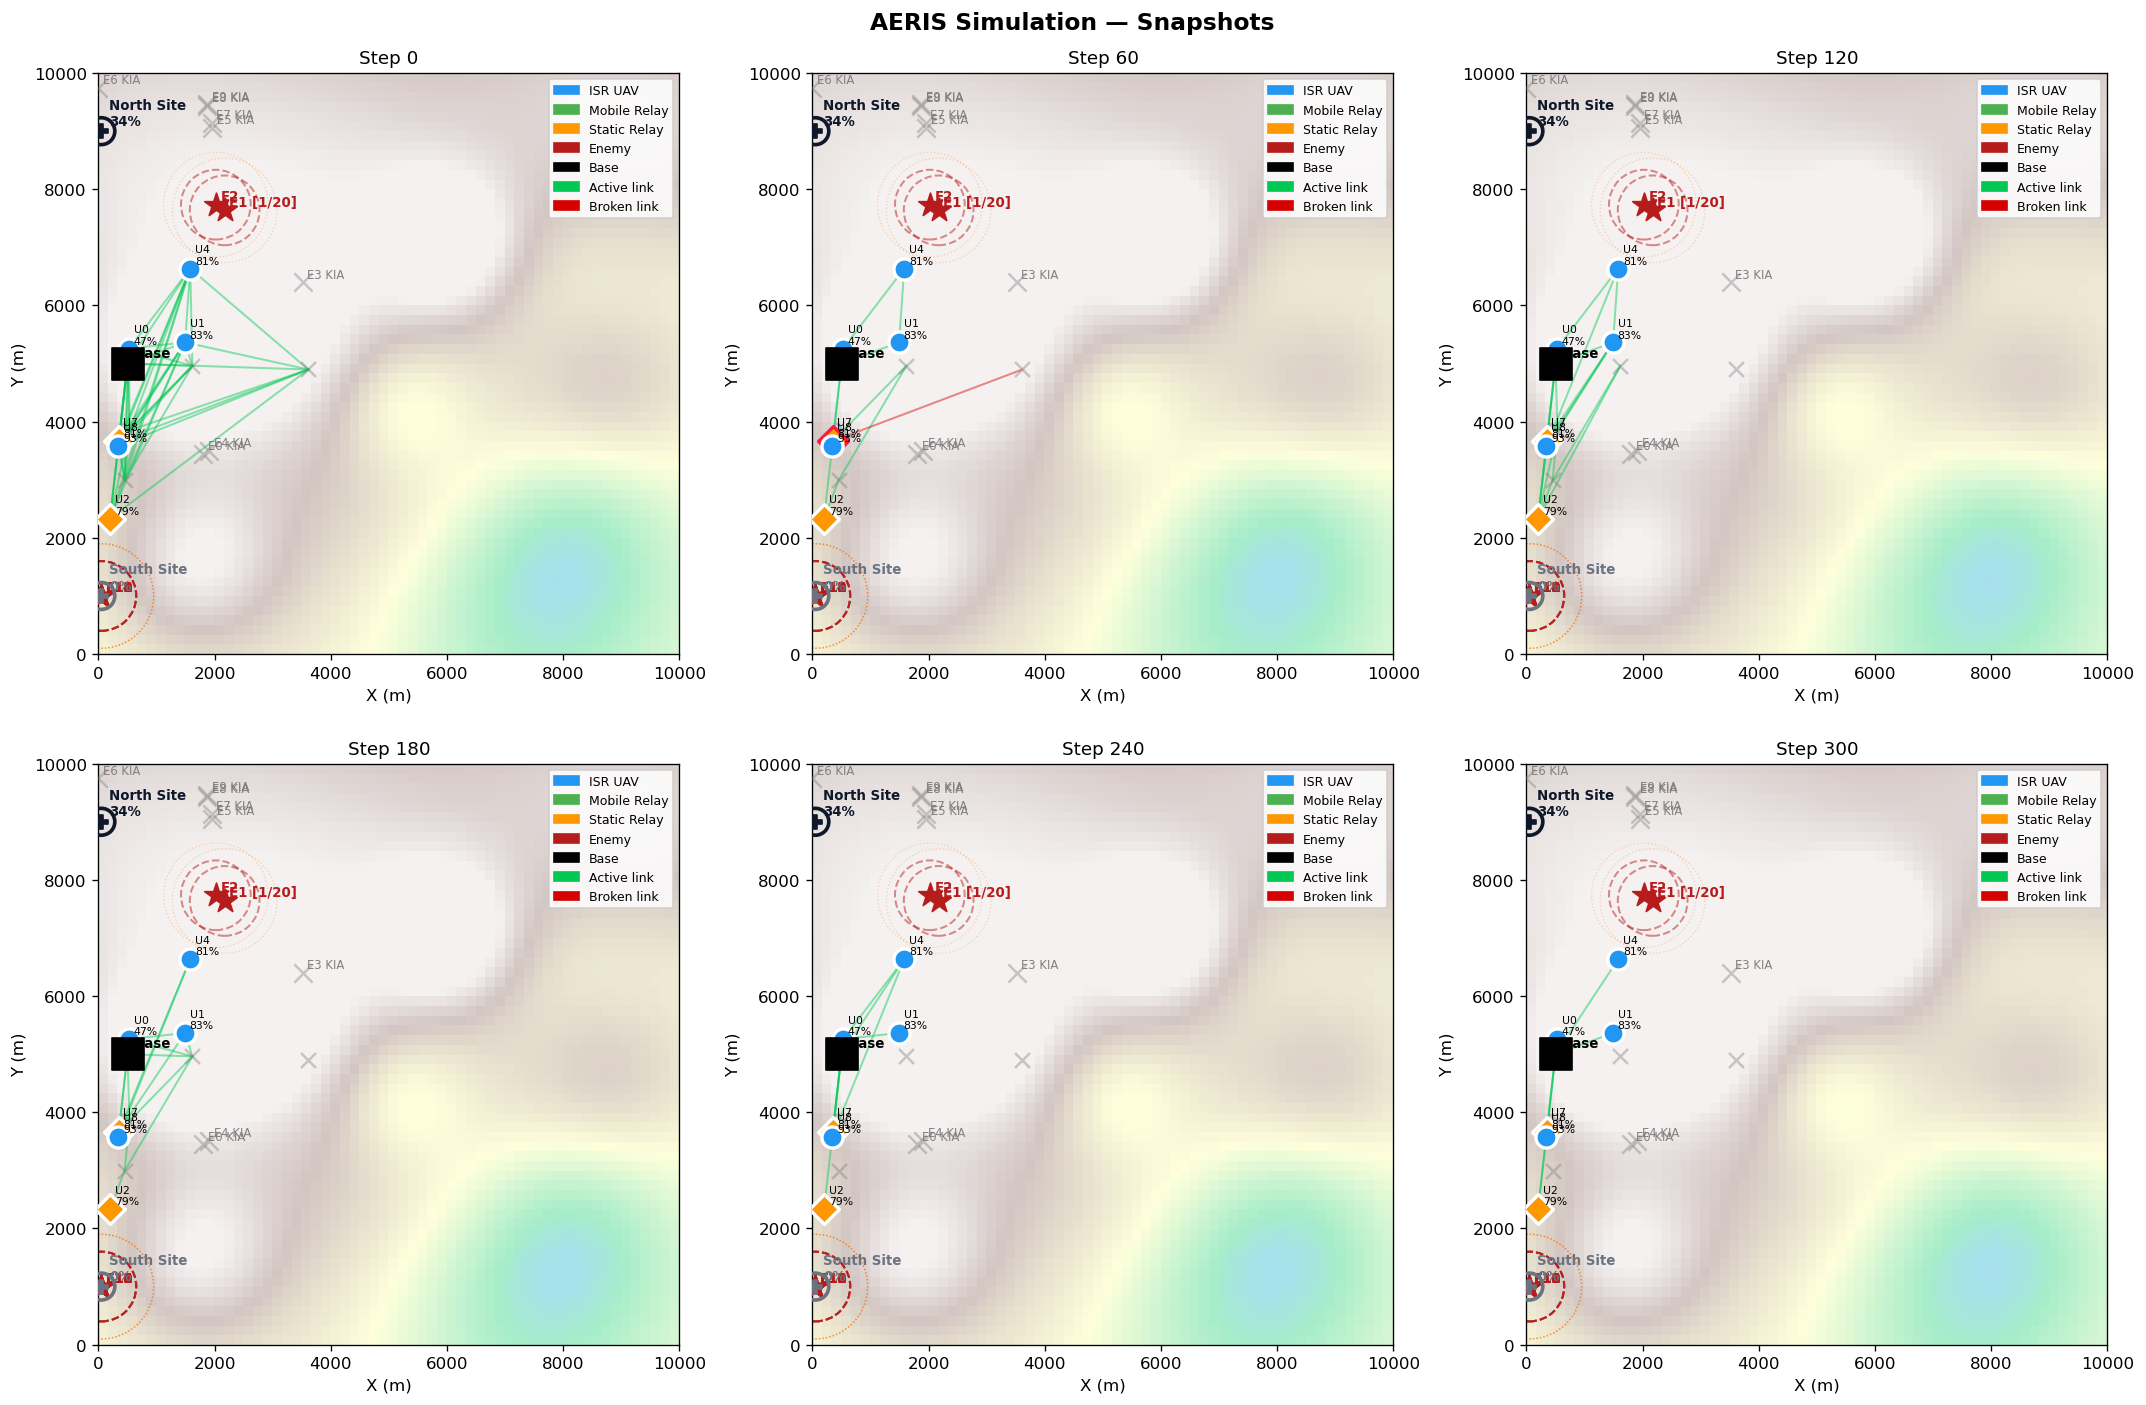
\includegraphics[width=0.92\textwidth]{aeris_dual_objective_snapshots.png}
    \caption{Dual-objective scenario snapshots. The north and south sites create
    a multi-axis defense problem that the original single-chain behavior could
    not address robustly.}
    \label{fig:dual_snapshots}
\end{figure*}

\subsection{Adaptive Branching Relay Chain}
The optimizer has been extended from a single relay chain to adaptive branching.
Enemies are clustered into north, center, and south bands. The optimizer then
allocates relay waypoints across active bands, allowing the UAV network to form
multiple communication branches rather than overcommitting to a single centerline
path.

\subsection{Objective Urgency Layer}
The optimizer now includes objective-aware urgency terms. Enemy groups targeting
secondary sites receive additional branch weight, and the scoring function
penalizes objective loss while rewarding objective health. The ISR reserve was
also increased so that more UAVs remain available for sensing rather than being
converted into relays too aggressively.

\subsection{Multi-Seed Benchmarking}
A new benchmark runner executes the same scenario across multiple random seeds
and reports mean, standard deviation, and interquartile ranges for key metrics.
This changed evaluation from one-off animations to statistically useful
comparisons.

\begin{figure*}[t]
    \centering
    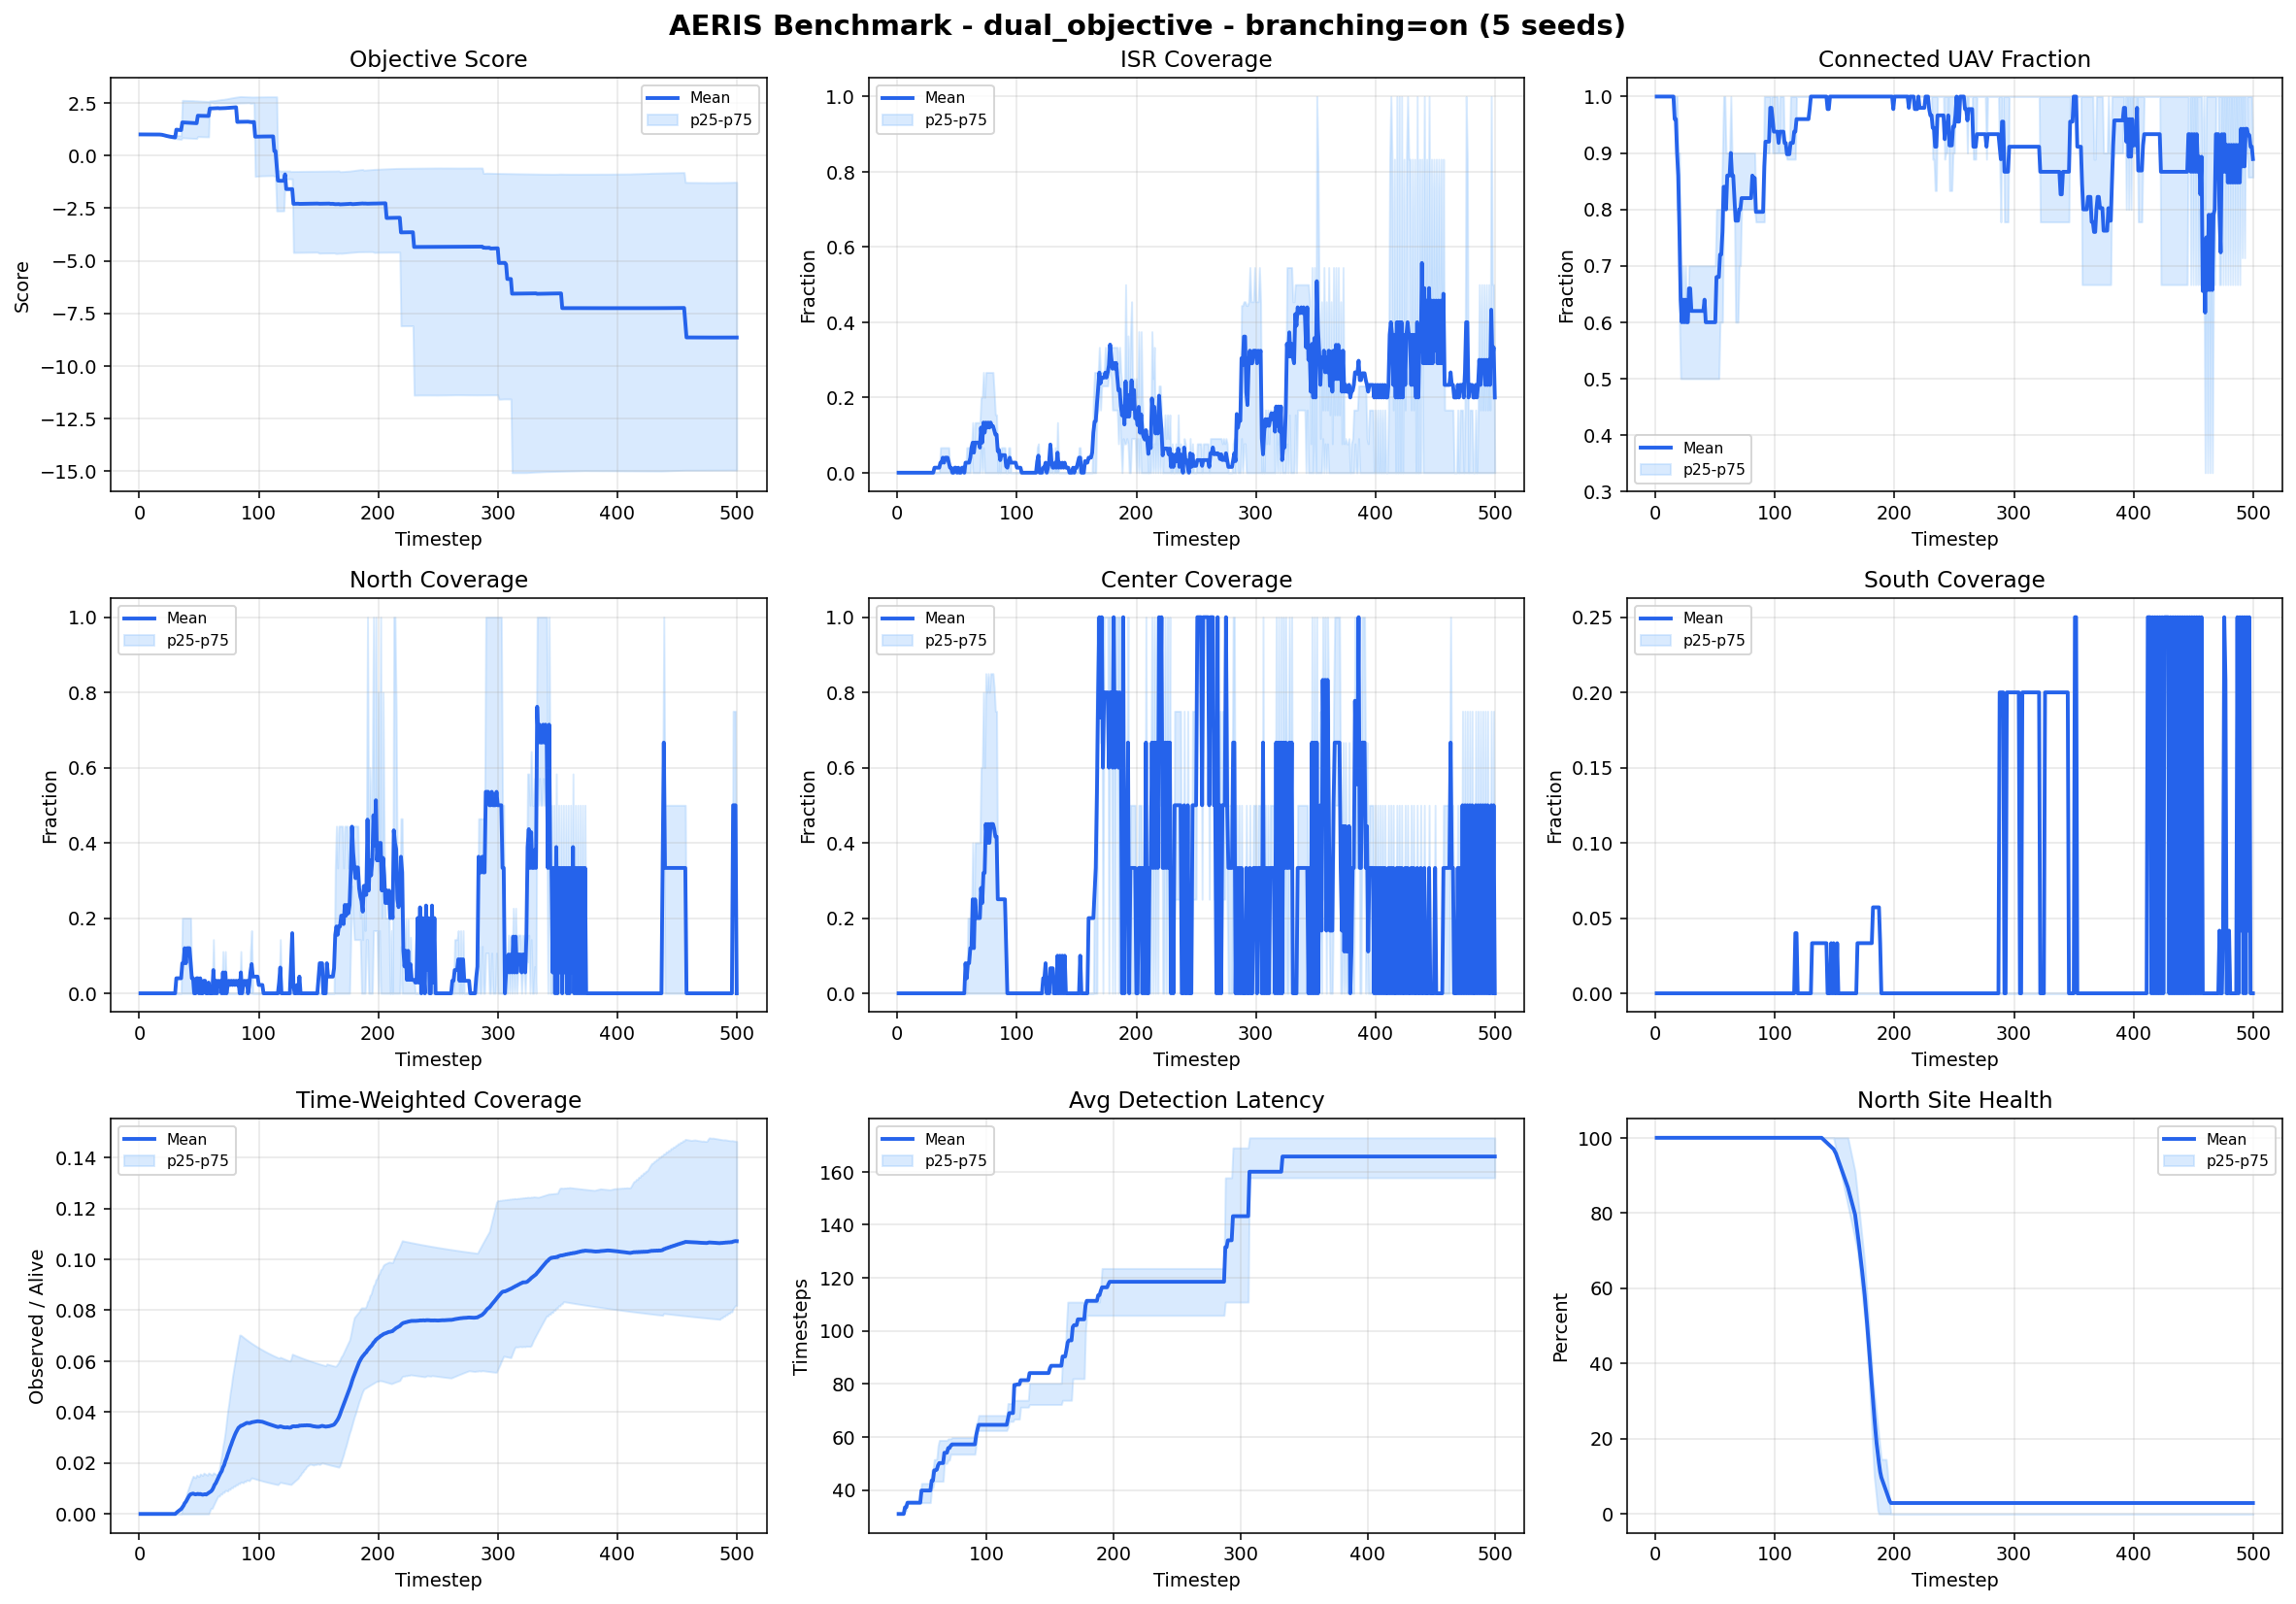
\includegraphics[width=0.92\textwidth]{benchmark_dual_on_5seed.png}
    \caption{Five-seed benchmark for the dual-objective scenario with adaptive
    branching enabled. Banded plots show seed-to-seed variability.}
    \label{fig:benchmark_branching}
\end{figure*}

\section{Current Experimental Findings}

\subsection{Branching Helps, But Does Not Yet Save the Sites}
Adaptive branching gives the simulator more believable multi-axis behavior, but
the north and south objectives still frequently reach zero health. This suggests
that the current policy can eventually strike enemies, but it does not detect and
hold coverage on objective-bound enemies early enough.

\subsection{Persistent ISR Watch Was Tested}
A persistent ISR watch experiment was added behind a configuration flag. The
idea was to hold ISR UAVs near the enemy-to-objective lanes so that flank
coverage would begin earlier. However, five-seed benchmarks showed that this
reduced performance. With persistent watch enabled, UAVs loitered too far from
the enemies or exposed themselves before the relay chain could support sustained
connected observation.

\begin{figure*}[t]
    \centering
    \begin{subfigure}{0.48\textwidth}
        \centering
        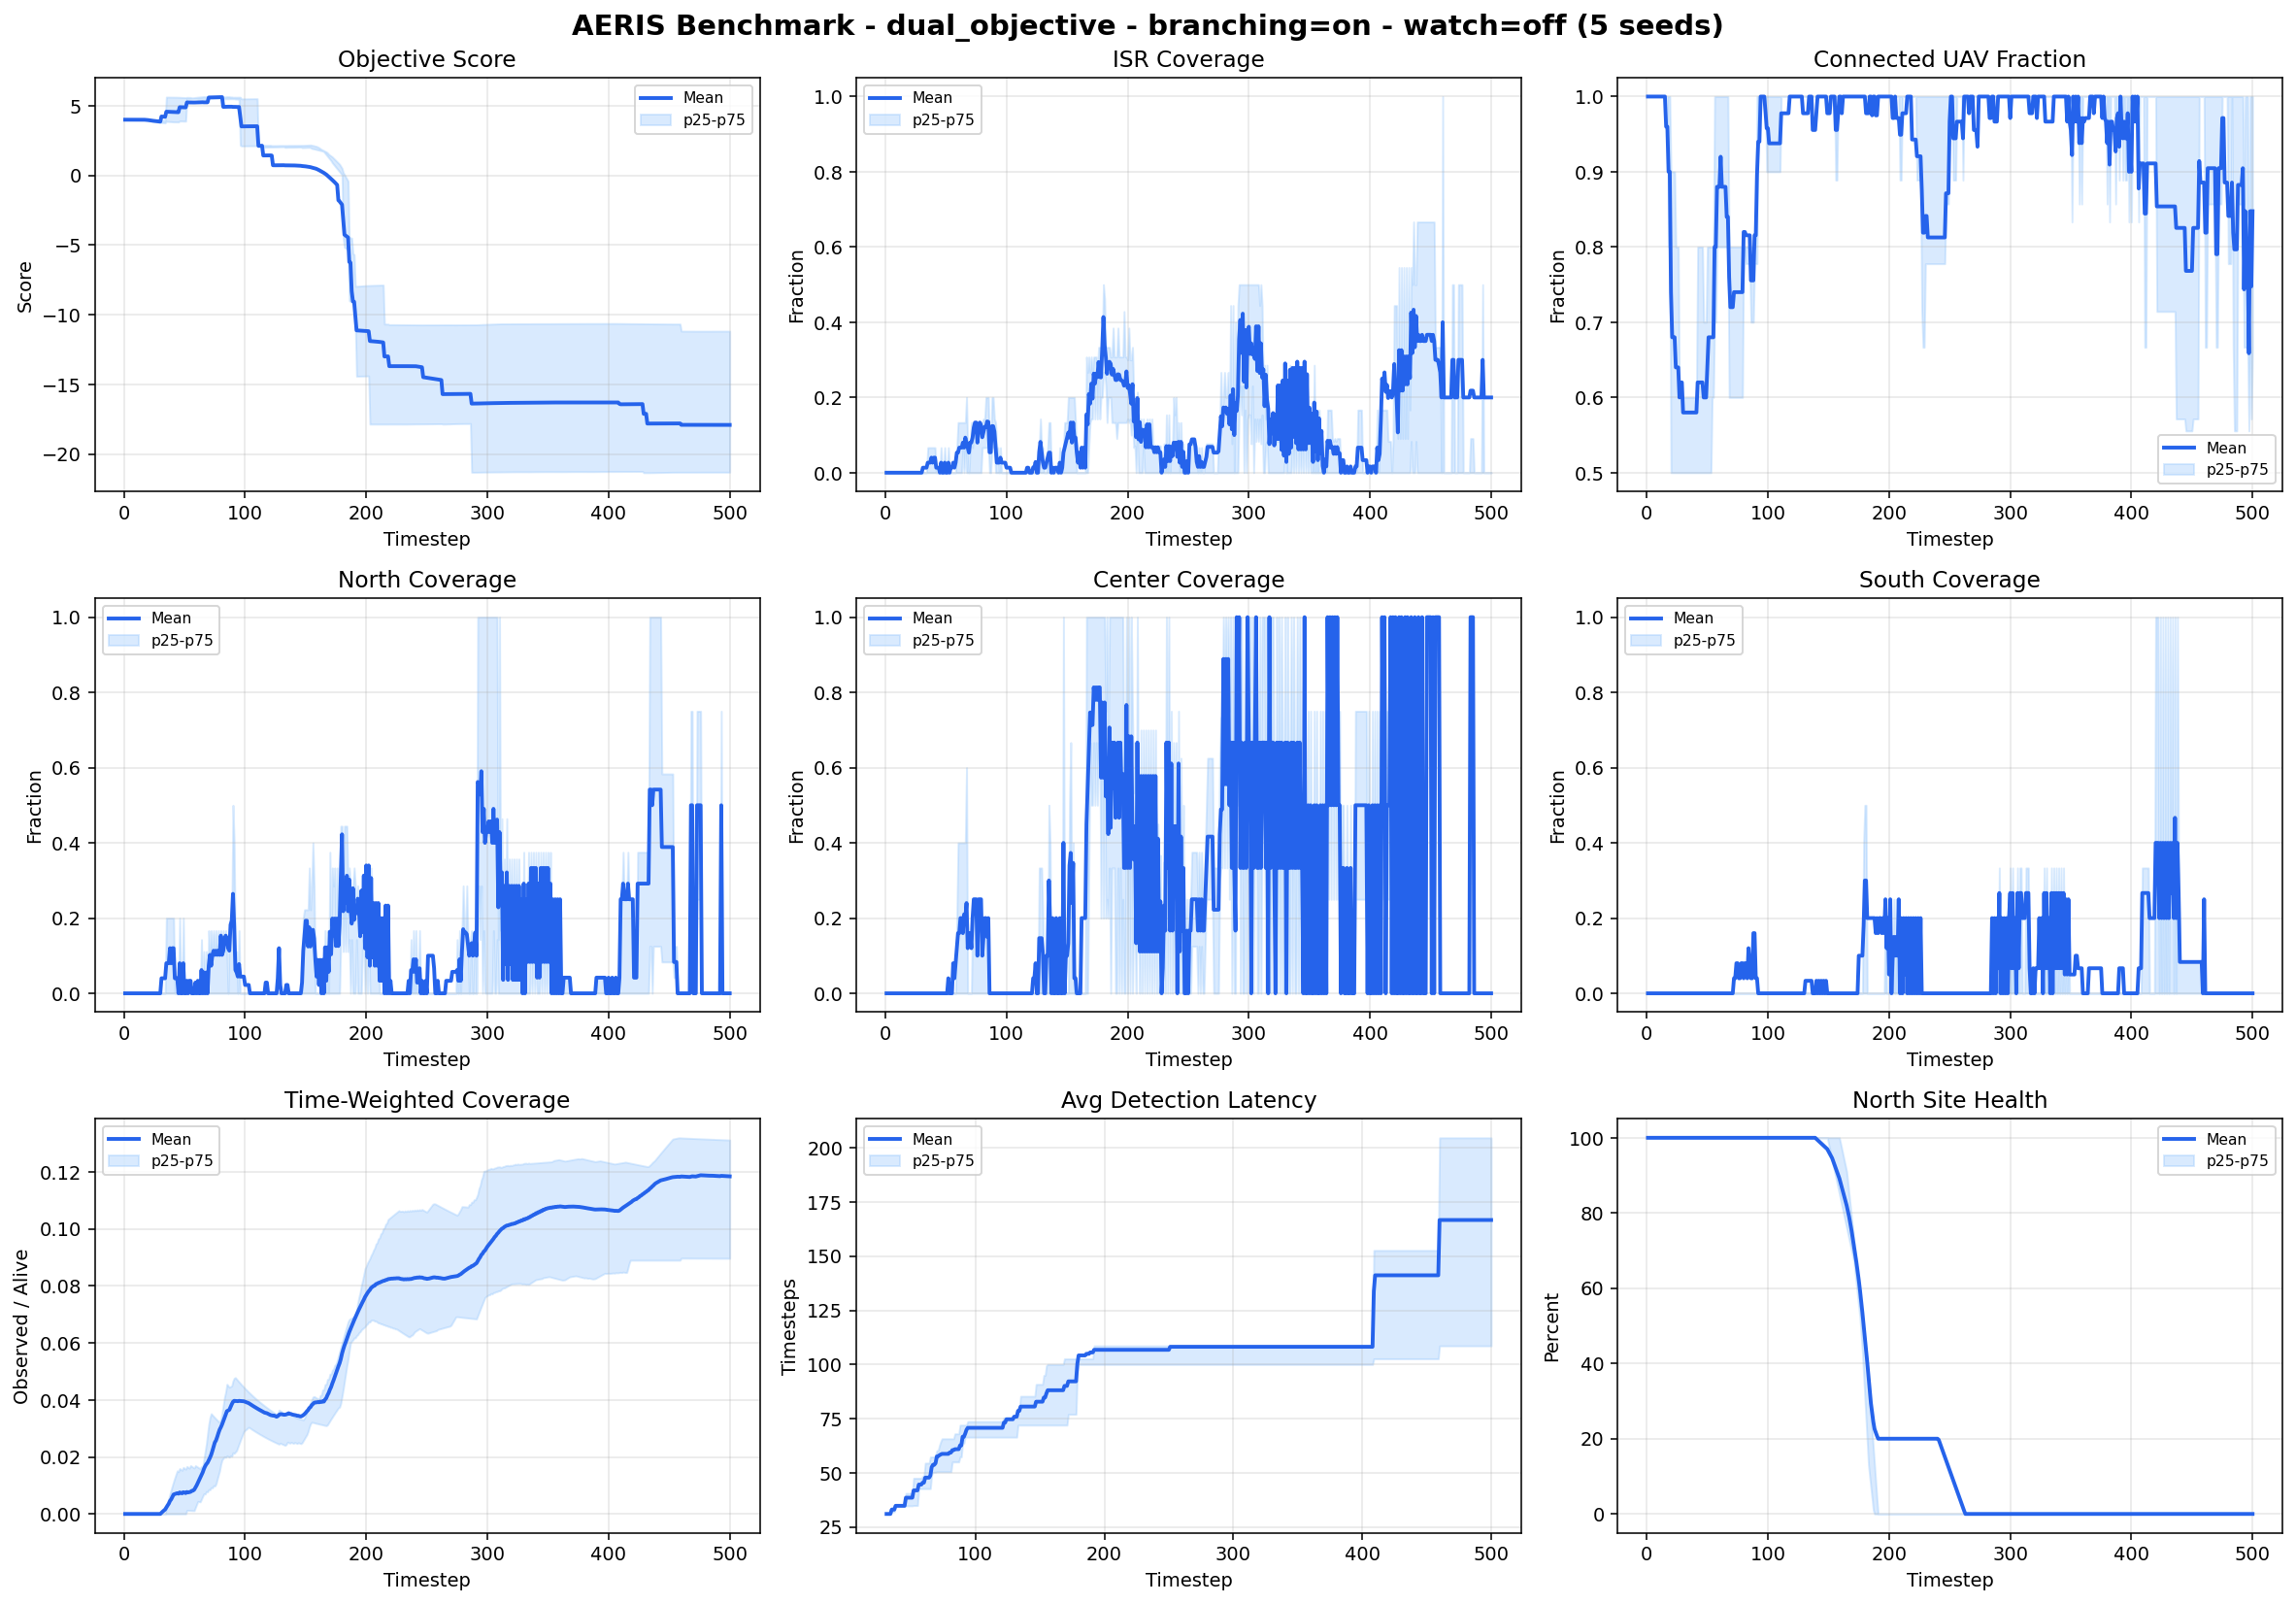
\includegraphics[width=\linewidth]{benchmark_watch_off_5seed.png}
        \caption{Persistent watch disabled.}
    \end{subfigure}
    \hfill
    \begin{subfigure}{0.48\textwidth}
        \centering
        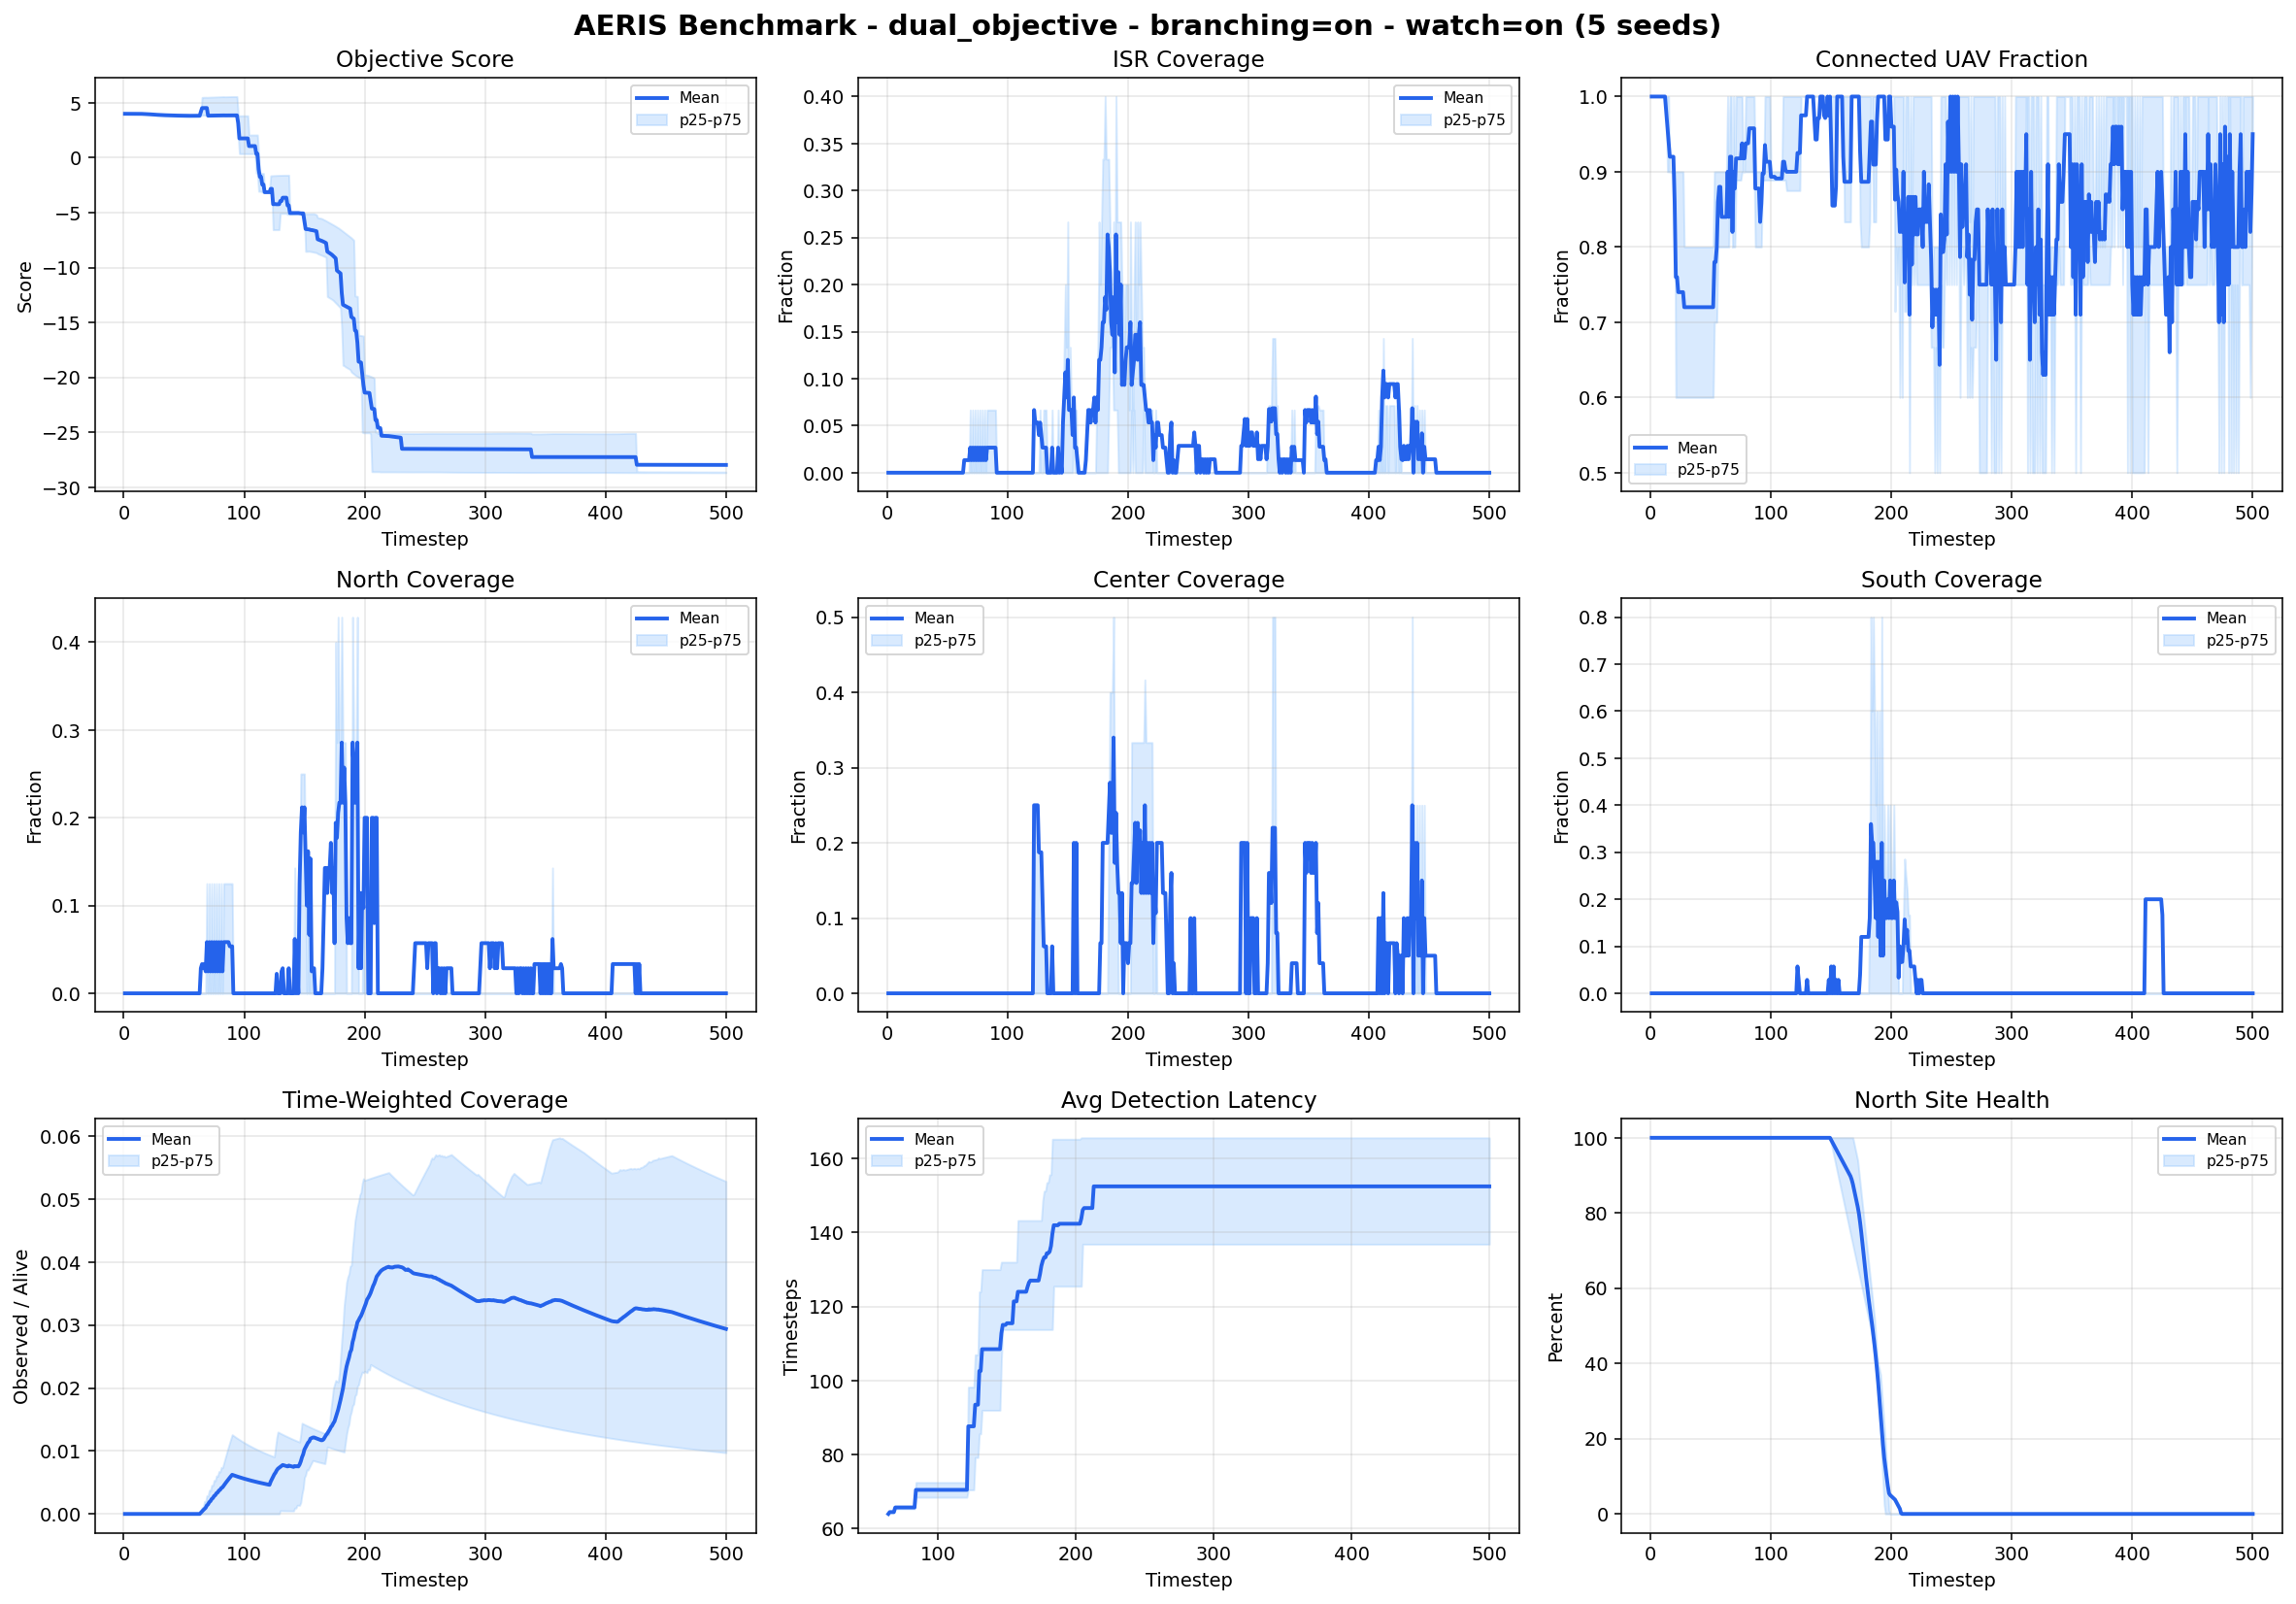
\includegraphics[width=\linewidth]{benchmark_watch_guarded_on_5seed.png}
        \caption{Persistent watch enabled.}
    \end{subfigure}
    \caption{Persistent ISR watch did not improve the current policy. It
    preserved the idea of defensive coverage, but delayed decisive enemy
    tracking and increased mission failure in benchmark runs.}
    \label{fig:persistent_watch}
\end{figure*}

\begin{table}[t]
    \centering
    \caption{Five-seed benchmark comparison for persistent ISR watch.}
    \label{tab:watch_results}
    \begin{tabular}{lcc}
        \toprule
        Metric & Watch Off & Watch On \\
        \midrule
        Final objective & -17.90 & -27.97 \\
        Total strikes & 9.40 & 0.20 \\
        UAVs alive & 7.00 & 4.20 \\
        Enemies remaining & 5.60 & 14.80 \\
        North site health & 0.00 & 0.00 \\
        South site health & 0.00 & 0.00 \\
        \bottomrule
    \end{tabular}
\end{table}

\section{What Has Changed Relative to the Proposal}

\begin{table*}[t]
    \centering
    \caption{Proposal-to-current implementation delta.}
    \label{tab:proposal_delta}
    \begin{tabular}{p{0.28\textwidth} p{0.32\textwidth} p{0.32\textwidth}}
        \toprule
        Proposal Component & Original Intent & Current Status \\
        \midrule
        Dynamic graph model
        & Model UAVs and base as nodes with communication links.
        & Implemented with per-step graph rebuild and connected component checks. \\
        \addlinespace
        Connectivity-constrained ISR
        & ISR observations only matter if transmitted to operator.
        & Implemented. Coverage requires connected ISR observation. \\
        \addlinespace
        Role switching
        & Switch between ISR, mobile relay, and static relay modes.
        & Implemented with promotion, static conversion, RTB, and recharge. \\
        \addlinespace
        FDIR behavior
        & Detect degraded connectivity and recover through role changes.
        & Implemented as heuristic recovery and relay chain maintenance. \\
        \addlinespace
        Optimization objective
        & Multiobjective score balancing ISR, connectivity, energy, workload, and switching.
        & Replaced with more diagnostic scoring: time-weighted coverage, latency, connectivity, losses, and objective health. \\
        \addlinespace
        Evaluation
        & Compare adaptive FDIR against simpler baselines.
        & Multi-seed benchmark runner added; current comparisons include branching, urgency, and watch-policy variants. \\
        \addlinespace
        Visual demonstration
        & Show UAVs dynamically switching roles.
        & Implemented with animations, snapshots, and metric dashboards. \\
        \bottomrule
    \end{tabular}
\end{table*}

\section{Next Steps}

\subsection{Step 1: Emergency Objective Intercept Mode}
The immediate next step is to replace passive persistent watch with an emergency
intercept policy. When an objective-bound enemy is close enough that it could
damage the site before a normal patrol detects it, the optimizer should assign a
connected ISR UAV to chase that enemy directly and hold observation until a
strike occurs. This is different from loitering near a watch point: the UAV
should prioritize sustained detection of the most urgent enemy.

\subsection{Step 2: Receding-Horizon Assignment}
The current optimizer is still mostly heuristic. A stronger next version should
score candidate assignments over a short horizon. At each step, the policy can
evaluate possible ISR-to-enemy and relay-to-waypoint assignments using predicted
objective damage, detection latency, connectivity risk, and battery cost. This
would make the behavior visibly more optimization-driven.

\subsection{Step 3: Objective-Aware Relay Placement}
Relay branches should not only aim at enemy centroids. They should place
waypoints that support the ISR positions needed to maintain observations on
urgent objective threats. In practice, this means relay placement should be
coupled to ISR tasking rather than planned independently.

\subsection{Step 4: Full Baseline Comparison}
The benchmark runner should be extended to compare:
\begin{itemize}
    \item no relay adaptation,
    \item single-chain relay behavior,
    \item adaptive branching,
    \item branching with urgency,
    \item branching with emergency intercept.
\end{itemize}
The final result should show whether each added autonomy layer improves north
and south coverage, lowers detection latency, preserves objective health, or
trades those gains against UAV survival.

\subsection{Step 5: Final Demo Narrative}
For the final presentation, the strongest story is no longer only that UAVs can
form a relay chain. The stronger story is that the system discovers the failure
mode of a naive relay chain, adds adaptive branching, then exposes the remaining
gap: objective-bound enemies require urgent sustained detection. The final demo
should show this progression visually using the animation, snapshot, and
benchmark outputs.

\section{Conclusion}
Since the proposal, AERIS has moved from a conceptual connectivity-constrained
ISR framework into a working simulation and benchmark environment. The core
proposal claims are now represented in code: graph connectivity, valid ISR
coverage, role switching, relay deployment, and FDIR-style recovery. The project
has also expanded beyond the original linear scenario into a dual-objective
multi-axis defense problem. The main unresolved challenge is that current
heuristic optimization can eventually suppress threats but does not yet preserve
undefended objectives. The next phase should therefore focus on emergency
intercept behavior and short-horizon assignment optimization so that the visual
demo shows not only adaptive motion, but measurable tactical improvement.

\end{document}
